\chapter{Project Management}
\label{ch:intro-pm}

%%%%%%%%%%%%%%%%%%%%%%%%%%%%%%%
\section{Project Structure and Responsibilities}

The LBNF Project is charged by Fermilab and DOE to design and construct conventional and technical facilities needed to support the DUNE Collaboration. LBNF is organized as a DOE/Fermilab project incorporating in-kind contributions from international partners. At this time, the major international partner is CERN, the European Organization for Nuclear Research. LBNF works closely with DUNE through several coordinating groups to ensure scientific direction and coordination for executing the LBNF Project such that the requirements of the program are met. 

LBNF works closely with SURF management to coordinate design and construction for the far site conventional facilities for the DUNE far detector. CERN is providing cryogenics equipment and engineering as part of the cryogenics infrastructure at SURF. The design and construction of LBNF is supported by other laboratories and consultants/contractors that provide scientific, engineering, and technical expertise.  A full description of LBNF Project Management is contained in the LBNF/DUNE Project Management Plan\cite{PMP-10770}.

LBNF coordinates with DUNE through regular technical team interactions between the two Projects as well as more formally through the Experiment-Facility Interface Group, where major decisions regarding interfaces and items affecting both Projects are made. In addition, the Projects use an integrated and coordinated project resource-loaded schedule and use a common configuration management system. 


\fixme{from CDR vol 3 ch 2}
 


LBNF consists of two major L2 subprojects, Far Site Facilities and Near Site Facilities, coordinated through a central Project Office located at Fermilab.  Each L2 Project consists of two large L3 subprojects corresponding to the conventional and technical facilities, respectively, at each site. The project organizational structure, which includes leadership from major partners, is shown in Figure 2 1.


\fixme{from CDR vol 1 4.2}

The LBNF Project team consists of members from Fermilab, CERN, South Dakota Science and Technology Authority (SDSTA), and BNL.  The team, including members of the Project Office as well as the L2 and L3 managers for the individual subprojects, is assembled by the Project Director. The Project team is shown to WBS Level~3 in Figure~\ref{fig:lbnf-org}. 
Line management for environment, safety and health, and quality assurance flows through the Project Director. 

Through their delegated authority and in consultation with major stakeholders, the L2 Project Managers determine which of their lower-tier managers will be Control Account Managers (CAMs) for the Project WBS. L2 and L3 Project Managers are directly responsible for generating and maintaining the cost estimate, schedule, and resource requirements for their subprojects and for meeting the goals of their subprojects within the accepted baseline cost and schedule. 

\begin{cdrfigure}[LBNF Work Breakdown Structure (WBS) to level 3]{lbnf-wbs}{LBNF Work Breakdown Structure (WBS) to level 3}
%  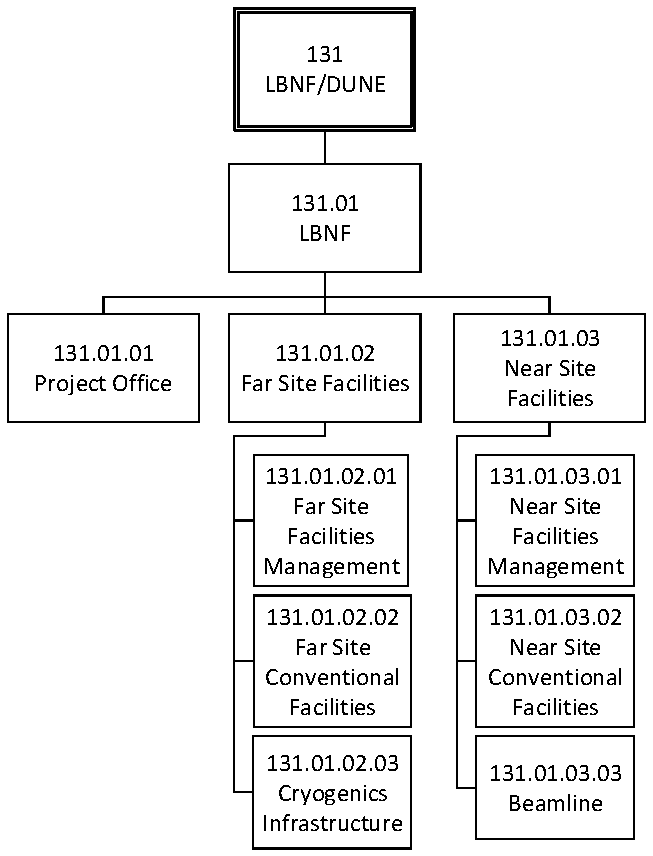
\includegraphics[width=0.8\textwidth]{lbnf-wbs-l3-nonames}
\end{cdrfigure}



\begin{cdrfigure}[LBNF organization]{lbnf-org}{LBNF organization}
%  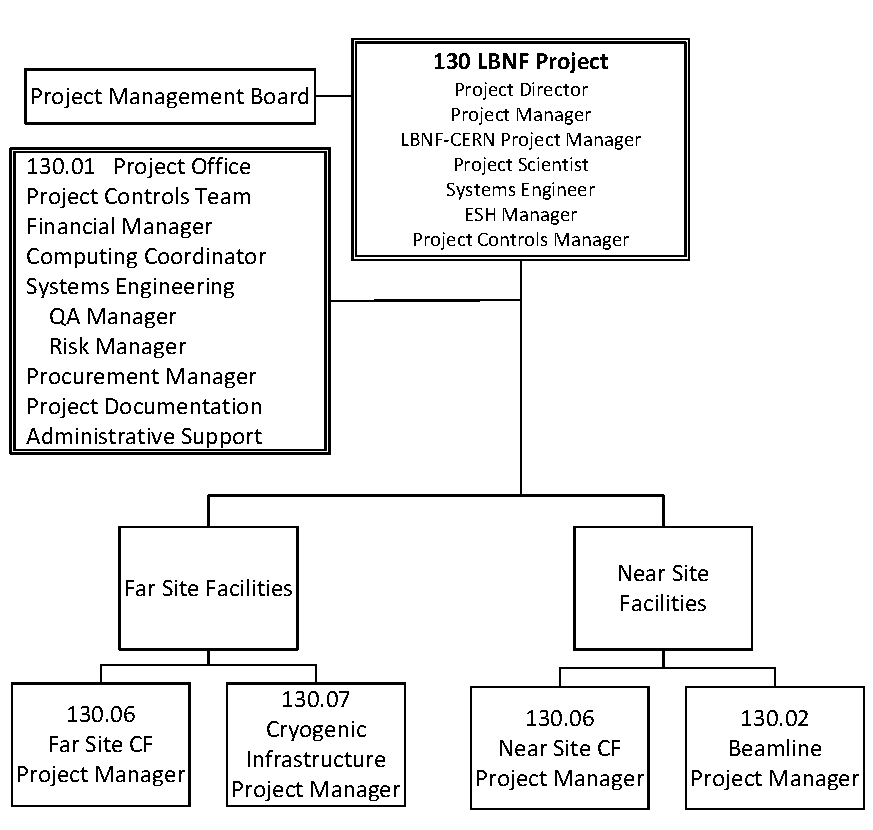
\includegraphics[width=0.8\textwidth]{lbnf-org}
\end{cdrfigure}

%%%%%%%%%%%%%%%%%%%%%%%%%%%%%%%
\section{SDSTA and SURF}

LBNF plans to construct facilities at SURF to house the DUNE far detector. SURF is owned by the state of South Dakota and managed by the SDSTA. 

Current SURF activities include operations necessary for allowing safe access to the 4850L of the former mine, which houses the existing and under-development science experiments. The DOE is presently funding SDSTA ongoing operations through Lawrence Berkeley National Laboratory (LBNL) and its SURF Operations Office through FY16; this is expected to change to funding through Fermilab starting in FY17. 

The LBNF Far Site Facilities Manager is also an employee of SDSTA and is contracted to Fermilab to provide management and coordination of the Far Site Conventional Facilities (CF) and Cryogenics Infrastructure subprojects. LBNF contracts directly with SDSTA for the design of the required CF at SURF; whereas the actual construction of the CF will be directly contracted from Fermilab. Coordination between SDSTA and the LBNF Project is necessary to ensure efficient operations at SURF. This will be facilitated via an agreement between SDSTA and Fermilab \fixme{new reference} that defines responsibilities and methods for working jointly on LBNF Project design and construction. A separate agreement will be written for LBNF Operations. 

%%%%%%%%%%%%%%%%%%%%%%%%%%%%%%%
\section{CERN}

The European Organization for Nuclear Research (CERN) is expected to significantly contribute to LBNF with technical components, required to support the deployment of the DUNE detectors and of the neutrino beamline. 

%%%%%%%%%%%%%%%%%%%%%%%%%%%%%%%
\section{Coordination within LBNF}

The LBNF Project organization is headed by the LBNF Project Director, who is also the Fermilab Deputy Director for LBNF; this person reports directly to the Fermilab Director. 

Within Fermilab's organization, two new divisions are being created to execute the Far Site Facilities and Near Site Facilities subprojects. The heads of these divisions will report to the LBNF Project Manager. 
Any personnel working more than half-time on these subprojects would typically be expected to become a member of one of these divisions, while other contributors will likely be matrixed in part-time roles from other Fermilab Divisions.  The heads of the other Fermilab Divisions work with the L1 and L2 project managers to supply the needed resources on an annual basis.  The management structure described above is currently being transitioned into and will not be fully in place until the Fall of 2015.  

The LBNF WBS defines the scope of the work. All changes to the WBS must be approved by the LBNF Project Manager prior to implementation. At the time of CD-1-Refresh, the LBNF WBS is in transition. Both the current and the post CD-1-R WBS is shown in Figure~\ref{fig:lbnf-wbs} \fixme{there will only be post-CD-1-R?} to demonstrate how the scope will map from one WBS to the other. 
SDSTA assigns engineers and others as required to work on specific tasks required for the LBNF Project at the SURF site. This is listed in the resource-loaded schedule as contracted work from Fermilab for Far Site CF activities. 
CERN and Fermilab are developing a common cryogenics team to design and produce the Cryogenics Infrastructure subproject deliverables for the far site. CERN provides engineers and other staff as needed to complete their agreed-upon deliverables.  
LBNF has formed several management groups with responsibilities as described below.

\textbf{Project Management Board:} LBNF uses a Project Management Board to provide formal advice to the Project Director on matters of importance to the LBNF Project as a whole. Such matters include (but are not limited to) those that
\begin{itemize}
\item have significant technical, cost, or schedule impact on the Project
\item have impacts on more than one L2 subproject
\item affect the management systems for the Project
\item have impacts on or result from changes to other Projects on which LBNF is dependent
\item result from external reviews or reviews called by the Project Director
\end{itemize}

The Management Board serves as the
\begin{itemize}
\item LBNF Change Control Board, as described in the Configuration Management Plan\cite{CMP-10760} 
\item Risk Management Board, as described in the Fermilab Risk Management Procedure for Projects~\cite{fnal-risk-mgmt} %Plan 
\end{itemize}

\textbf{Beamline Technical Board:} The role of the LBNF Beamline Technical Board (TB) is to provide recommendations and advice to the Beamline Project Manager on important technical decisions that affect the design and construction of the Beamline. The members of the Technical Board must have knowledge of the Project objectives and priorities in order to perform this function. The Beamline Project Manager chairs the Beamline TB. The Beamline Project Engineer is the Scientific Secretary of the Board and co-chairs the Beamline TB as needed. 

\textbf{FSCF Neutrino Cavity Advisory Board:} The Far Site CF (FSCF) Project has engaged three international experts in hard rock underground construction to advise it periodically through the design and construction process regarding excavation at SURF. The Board meets at the request of the FSCF-PM, generally on site to discuss specific technical issues. The Board produces a report with its findings and conclusions for Project information and action. 

%%%%%%%%%%%%%%%%%%%%%%%%%%%%%%%%%%%%%%%%%%%%%%%%%%%%%
\section{LBNF/DUNE Advisory and Coordinating Structures}
\label{sec:lbnf-dune-interface}

\fixme{do we need this? I did not pull in content.}


%%%%%%%%%%%%%%%%%%%%%%%%%%%%%%%%%%%%%%%%%%%%%%%%%%%%%%%%%%%%%%%%%%%
\section{Work Breakdown Structure}
\label{sec:fs-pm-wbs}


text

%%%%%%%%%%%%%%%%%%%%%%%%%%%%%%%%%%%%%%%%%%%%%%%%%%%%%%%%%%%%%%%%%%%
%%%%%%%%%%%%%%%%%%%%%%%%%%%%%%%%%%%%%%%%%%%%%%%%%%%%%%%%%%%%%%%%%%%
\section{Reference stuff to remove}

Refer to figure as Figure~\ref{fig:label} and uncomment once there's a real filename to enter.

\begin{cdrfigure}[short]{label}{long}
%\includegraphics[width=0.8\textwidth]{filename}
\end{cdrfigure}

Here's a sample table; refer to it as Table~\ref{tab:label}.

\begin{cdrtable}[short]{lcc}{label}{long }
Physics milestone & Exposure \ktMWyr{} & Exposure \ktMWyr{}\\ \rowtitlestyle
  & (reference beam) & (optimized beam) \\ \toprowrule 
  $1^\circ$ $\theta_{23}$ resolution ($\theta_{23} = 42^\circ$) & 70  &  45\\ \colhline
  CPV at $3\sigma$ ($\delta_{\rm CP} = +\pi/2$)  & 70 & 60 \\ \colhline
  CPV at $3\sigma$ 75\% of \deltacp & 1320 & 850\\ 
\end{cdrtable}




